\documentclass{article}


\usepackage[margin=1in]{geometry}
\usepackage{microtype}
\usepackage[utf8]{inputenc}
\usepackage[T1]{fontenc}
\usepackage{amsmath}
\usepackage{amssymb}
\usepackage{tikz}
\usetikzlibrary{arrows}
\usepackage[printwatermark]{xwatermark}

%\newwatermark[allpages,color=blue!10,angle=45,scale=1.6,xpos=0,ypos=0]{DRAFT-Joseph Tabadero}
%\usepackage{xcolor}
%\usepackage{graphicx}

\newenvironment{solution}{\paragraph{Solution:}}{\hfill$\blacksquare$}



\newcommand{\abs}[1]{\ensuremath{\lvert #1\rvert}}
\newcommand{\degre}{\ensuremath{^\circ}}

\usetikzlibrary{positioning, decorations}
\makeatletter
\tikzset{
	distance from start/.code={%
		\pgfgetpath\currentpath\pgfprocessround{\currentpath}{\currentpath}%
		\pgf@decorate@parsesoftpath{\currentpath}{\currentpath}%
		\pgfmathparse{#1/\pgf@decorate@totalpathlength}\tikzset{pos=\pgfmathresult}},
	distance from end/.code={%
		\pgfgetpath\currentpath\pgfprocessround{\currentpath}{\currentpath}%
		\pgf@decorate@parsesoftpath{\currentpath}{\currentpath}%
		\pgfmathparse{1-(#1/\pgf@decorate@totalpathlength)}\tikzset{pos=\pgfmathresult}}
}

\title{Solutions to Part I of 17th PMO (Area Level)}
\author{Joseph S. Tabadero, Jr.}
\date{\today}



\begin{document}

\maketitle
	
\section*{Notations}

\begin{tabular}{rl}
	$AB$ & The segment $AB$ or the length of the segment $AB$. The usage is easily seen in context\\
	$[ABC]$ & The area of the region (triangle) $ABC$.\\
	$\angle BDA$ & The angle or the measure ($m\angle$) of the angle $BDA$.
\end{tabular}



\section{PART I.}

\begin{enumerate}
	\item What is the fourth smallest positive integer having exactly 4 positive integer divisors, including 1 and itself?
	
	\begin{solution}
		The answer provided by PMO is 14. We can get this result if we follow the folloing solution:
		\begin{align}
			1\times 2\times 2 &= 4\\
			1\times 2 \times 3 & = 6\\
			1\times 2\times 5 & = 10\\
			1\times 2\times 7 & = 14
		\end{align}
		But I fail to see why 4 is included since 2 is a divisor of multiplicity 2. All the others have unique divisors. The four smallest positive integers having exactly 4 positive integer divisors should have been: 6, 10, 14, 15. That is, the answer should have been $15 = 1\times 3\times 5$.
	\end{solution}


	\item Let $f(x)=a^x-1$. Find the largest value of $a>1$ so that if $0\leq x\leq 3$, then $0\leq f(x)\leq 3$.
	
	\begin{solution}
		Since $a>1$, $f(x)=a^x-1$ is an increasing function, which means that  $f(3)=3$. That is $a^3-1=3\implies a^3=4\implies a=\sqrt[3]{4}$.
	\end{solution}


	\item Simplify the expression $\left(1+\dfrac{1}{i}+\dfrac{1}{i^2}+\cdots+\dfrac{1}{i^{2014}}\right)^2$.
	
	
	\begin{solution}
		We note that
		\begin{align*}
			\frac{1}{i}&=\frac{1}{i}\cdot\frac{i}{i}=-i\\
			\frac{1}{i^2}&=\frac{1}{i^2}=\frac{1}{-1}=-1\\
			\frac{1}{i^3}&=\frac{1}{i^2}\cdot\frac{i}{i}=i\\
			\frac{1}{i^4}&=1
		\end{align*}
		and in general, it can be shown that
		\begin{align*}
		\dfrac{1}{i^{4n+1}}&=-i\\
		\dfrac{1}{i^{4n+2}}&=-1\\
		\dfrac{1}{i^{4n+3}}&=i\\
		\dfrac{1}{i^{4n}}&=1
		\end{align*}
		So that
		\begin{equation*}
		\left(1+\dfrac{1}{i}+\dfrac{1}{i^2}+\cdots+\dfrac{1}{i^{2014}}\right)^2=(1-i-1+i+\cdots 1-i-1)^2=-1
		\end{equation*}
	\end{solution}

	\item Find the numerical value of $(1-\cot 37^\circ)(1-\cot 8^\circ)$/
	
	\begin{solution}
		We know that $\cot 45^\circ=1$. We recall the identity $cot(x+y)=\dfrac{\cot x\cot y-1}{\cot x+\cot y}$. Letting $x=37^\circ$ and $y=8^\circ$ then $1=\dfrac{\cot x\cot y-1}{\cot x+\cot y}$ or $\cot x+\cot y=\cot x\cot y-1$ from which we have $1=\cot x\cot y - \cot x-\cot y$. Now, $(1-\cot x)(1-\cot y)=1\underbrace{-\cot x-\cot y+\cot x\cot y}_{1}=1+1$.
	\end{solution}

	\item Triangle $ABC$ has right angle at $B$, with $AB=3$ and $BC=4$. If $D$ and $E$ are points on $AC$ and $BC$, respectively, such that $CD=DE=\frac{5}{3}$, find the perimeter of quadrilateral $ABED$.
	
	\begin{solution} Consider the figure below.
		
	\definecolor{uuuuuu}{rgb}{0.26666666666666666,0.26666666666666666,0.26666666666666666}
	\begin{tikzpicture}[line cap=round,line join=round,>=triangle 45,x=1cm,y=1cm]
	\clip(-0.5,-0.5) rectangle (4.5,3.5);
	\draw [line width=2pt] (0,3) -- (0,0) -- (4,0) -- cycle;
	\draw [line width=2pt] (0,3)-- (0,0);
	\draw [line width=2pt] (0,0)-- (4,0);
	\draw [line width=2pt] (4,0)-- (0,3);
	\draw [line width=2pt] (2.6666666666666665,1)-- (1.333333333333333,0);
	\draw [line width=2pt] (2.072,0.404) -- (1.928,0.596);
	\draw [line width=2pt] (4,0)-- (2.6666666666666665,1);
	\draw [line width=2pt] (3.2613333333333325,0.404) -- (3.405333333333334,0.596);
	\draw [line width=2pt,dash pattern=on 1pt off 1pt] (2.6666666666666665,1)-- (2.6666666666666665,0);
	\begin{scriptsize}\draw [fill=black] (0,3) circle (2.5pt);
	\draw[color=black] (0,3) node [above] {$A$};
	\draw [fill=black] (0,0) circle (2.5pt);
	\draw[color=black] (0,0) node[below left] {$B$};
	\draw [fill=black] (4,0) circle (2.5pt);
	\draw[color=black] (4.28,0.09) node {$C$};
	\draw [fill=black] (2.6666666666666665,1) circle (2pt);
	\draw[color=black] (2.67,1.17) node[above] {$D$};
	\draw [fill=black] (4,0) circle (2pt);
	\draw [fill=black] (1.333333333333333,0) circle (2pt);
	\draw[color=black] (1.08,0) node [below] {$E$};
	\draw [fill=uuuuuu] (1.3333333333333333,2) circle (2pt);
	\draw [fill=uuuuuu] (2,0.5) circle (2pt);
	\draw [fill=uuuuuu] (2.6666666666666665,0) circle (2pt);
	\draw[color=uuuuuu] (2.67,0) node [below] {$G$};
	\end{scriptsize}
	\end{tikzpicture}
	
	$CD$ has length $\frac{5}{3}$ or $\frac{1}{3}$ the length of $CA$. Draw segment $DG\perp BC$. Then $DG$ is $\frac{1}{3}$ of $AB$, or $DG=1$. Also, $CG=\frac{1}{3}\cdot BC=\frac{4}{3}$ so that $EC=\frac{8}{3}$ and $BE=4-\frac{8}{3}=\frac{4}{3}$. Therefore, the perimeter of $ABED$ is $\frac{4}{3}+\frac{5}{3}+\frac{10}{3}+3=9\frac{1}{3}$.
	
	\end{solution}

	
	\item Rationalize the denominator of $\dfrac{6}{\sqrt[3]{4}+\sqrt[3]{16}+\sqrt[3]{64}}$ and simplify.
	
	\begin{solution}
		\begin{align}
			\dfrac{6}{\sqrt[3]{4}+\sqrt[3]{16}+\sqrt[3]{64}} & = \frac{6}{\sqrt[3]{4}+2\sqrt[3]{2} + 4}\label{eq:5}
		\end{align}
		Letting $x=2$ and $y=\sqrt[3]{2}$, we can see that $4+2\sqrt[3]{2} + \sqrt[3]{4}=x^2 +xy+y^2$, which we multiply by $(x-y)=2-\sqrt[3]{2}$ to get $x^3-y^3=8-2=6$. Therefore, multiplying \eqref{eq:5} by $\dfrac{2-\sqrt[3]{2}}{2-\sqrt[3]{2}}$, we get $\dfrac{6(2-\sqrt[3]{2})}{6}=2-\sqrt[3]{2}$.
	\end{solution}

	\item Find the area of the triangle having vertices $A(10,-9)$, $B(19,3)$, and $C(25,-21)$.
	
	\begin{solution}
		You can use the shoelace formula which states that if $A(x_1, y_1)$, $B(x_2,y_2)$, and $C(x_3,y_3)$ are the coordinates of the vertices of the triangle, then the area of the triangle is
		\begin{equation}
			[ABC] = \frac{1}{2}\left\lvert \det \begin{bmatrix}
			x_1 & x_2 & x_3\\
			y_1 & y_2 & y_3\\
			1 & 1 & 1
			\end{bmatrix} \right\rvert.
		\end{equation}
		But this is not very intuitive. We can derive a special case of the shoelace formula. The special case states that if one of the vertices is at the origin, and the coordinates of the other two vertices are $(a,b)$ and $(c,d)$, then the area of the triangle is $\frac{1}{2}\lvert ad-bc\rvert$.
		
		To see this, consider the case below. Here, we fixed one of the vertices at $(0,0)$. The area of the shaded triangle is simply the area of the rectangle minus the areas of the unshaded triangles. It is easy to show that it is equal to $\frac{1}{2}(ad-bc)$ in this case.
		
		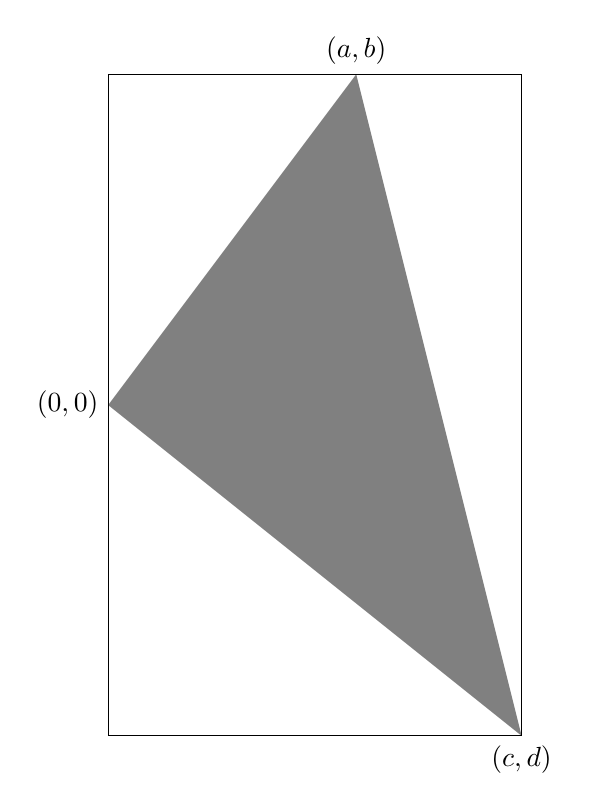
\begin{tikzpicture}[scale=0.35]
			\fill [color=gray] (10,-9) -- (19,3) -- (25,-21) --cycle;
			\draw (10,-21) -- (25,-21) -- (25,3) -- (10,3) --cycle;
			\node at (10,-9) [left] {$(0,0)$};
			\node at (19,3) [above] {$(a,b)$};
			\node at (25,-21) [below] {$(c,d)$};
		\end{tikzpicture}
		
		To apply this to our current problem, we simply translate the origin to $A(10,-9)$ so that the new coordinates become $A'(0,0)$, $B'(9,12)$, and $C'(15,-12)$. Then using the special case of the shoestring formula, we have
		\begin{equation*}
			[ABC]=[A'B'C']=\frac{1}{2}\abs{(9\times -12)-(12\times15)}=144.
		\end{equation*}
	\end{solution}

	\item How many ways can 6 boys and 6 girls be seated in a circle so that no two boys sit next to each other?
	
	\begin{solution}
		The 6 boys can pair up with the 6 girls in $6!$ ways in such a way that no two boys (hence no two girls) will sit next to each other. However, each pair can only be arranged $5!$ ways in a circle. Therefore, there are $6!5!=86400$ ways that the desired seating arrangement can be done.
	\end{solution}

	\item Two numbers $p$ and $q$ are both chosen randomly (and independently of each other) form the interval $[-2,2]$. Find the probability that $4x^2+4px+1-q^2=0$ has imaginary roots.
	
	\begin{solution}
		The sample space is the square region defined by the diagonal $(-2,-2)$ and $(2,2)$, that is the region $[-2,2]\times [-2,2]=\{(p, q): p\in [-2,2], q\in [-2,2] \}$, which has an area of 16. The event that $4x^2+4px+1-q^2=0$ will have imaginary roots occurs when the discriminant $b^2-4ac=16p^2-16(1-q^2)<0$, that is when $p^2+q^2<1$, whih is a circular region centered at $(0,0)$, radius $1$, and area $\pi$. Therefore, the probablity that $4x^2+4px+1-q^2=0$ will have imaginary roots is equal to the area of the circle over the area of the square or $\frac{\pi}{16}$.
	\end{solution}

	\item In $\triangle ABC$, $\angle A=80^\circ$, $\angle B=30^\circ$, and $\angle C=70^\circ$. Let $BH$ be an altitude of the triangle. Extend $BH$ to a point $D$ on the other side of $AC$ so that $BD=BC$. Find $\angle BDA$.
	
	\begin{solution} Consider the figure below.
		
		\includegraphics[width=0.5\linewidth]{PMO17-5}
		
		By the isosceles triangle theorem, we have $BD=BC$ and $\angle BDC=\angle BCD$. Since $\angle CHB$ is a right angle, we have $m\angle CBH = 20$. Therefore, $m\angle BDC=m\angle BCD=80$. Consequently, we have $m\angle HCD = m\angle HBA = 10$. Therefore, by $AA$ theorem, we have $\triangle DHC\sim \triangle AHB$. We will now show that $\triangle DHA\sim \triangle CHB$ and therefore conclude that $m\angle BDA = m\angle HDA = 70$. To show this, we only need to show that corresponding adjacent sides are proportional since the included angles $\angle DHA$ and $\angle CHB$ are already congruent. That is,
		\begin{equation}\label{eq:10}
			\frac{DH}{HC} = \frac{HA}{HB}
		\end{equation}
		But since  $\triangle DHC\sim \triangle AHB$, we have their corresponding sides proportional, in particular
		\begin{equation}
			\frac{DH}{HA} = \frac{HC}{HB}
		\end{equation}
		from which \eqref{eq:10} is easily derived.
	\end{solution}

	\item Find all integer values of $n$ that will make $\dfrac{6n^3-n^2+2n+32}{3n+1}$ an integer.
	
	\begin{solution}
		By long division, we have
		\begin{equation}\label{eq:11}
			\frac{6n^3-n^2+2n+32}{3n+1} = 2n^2-n+1 + \frac{31}{3n+1}
		\end{equation}
		For \eqref{eq:11} to be an integer, we must have $(3n+1) \mid 31$. But since 31 is prime, the only divisors of 31 are 1 and itself. That is, either $3n+1=1\implies n=0$ or $3n+1=31\implies n=10$. Therefore, the desired values are $0$ and $10$.
	\end{solution}

	\item Suppose that the function $y=f(x)$ satisfies $1-y=\dfrac{9e^x + 2}{12e^x+3}$. If $m$ and $n$ are consecutive integers so that $m<\dfrac{1}{y}<n$ for all real $x$, find the value of $mn$.
	
	\begin{solution}
		Solving $1-y=\dfrac{9e^x + 2}{12e^x+3}$ for $y$, we have
		\begin{equation}
			y=\dfrac{3e^x+1}{12e^x+3}=\cfrac{3+\cfrac{1}{e^x}}{12+\cfrac{3}{e^x}}.
		\end{equation}
		Note that $y\to \frac{1}{4}$ as $x\to+\infty$ or as $x\to -\infty$ and that $y\to \dfrac{4}{15}$ as $x\to 0$. This means that $\dfrac{1}{4} < y < \dfrac{4}{15}$ or $\dfrac{15}{4}<\dfrac{1}{6}<4$. But $3<\dfrac{15}{4}$ so that $m=3$ and $n=4$. Therefore, $mn=12$.
	\end{solution}

	\item The product of the two roots of $\sqrt{2014}\, x^{\log_{2014}x} = x^{2014}$ is an integer. Find its units digit.
	
	\begin{solution} We have the following derivations
		\begin{align*}
			\sqrt{2014}\, x^{\log_{2014}x} &= x^{2014}\\
			\iff 2014^{1/2}x^{\log_{2014}x} & = x^{2014}\\
			\iff \log_{2014}2014^{1/2} + \log_{2014} x^{\log_{2014}x} & = \log_{2014}x^{2014}\\
			\iff \frac{1}{2} + (\log_{2014}x)^2& = 2014\log_{2014}x
		\end{align*}
		Letting $y=\log_{2014}x$, and completing squares, we easily get
		\begin{equation}
			\log_{2014} x_{1,2} = 1007\pm\sqrt{\frac{1007^2-2}{2}}\label{eq:13}
		\end{equation}
		Solving \eqref{eq:13} for $x$, we get
		\begin{equation}
			x_{1,2} = 2014^{1007\pm\sqrt{\frac{1007^2-2}{2}}}.
		\end{equation}
		Therefore, the product of the two roots is simply $2014^{2014}$. Since 2014 ends in 4, the odd powers will end in 4 and the even powers will end in 6. Therefore, $2014^{2014}$ will have 6 as its digits place.
	\end{solution}

	\item In how many ways can Alex, Billy, and Charles split 7 identical marbles among themselves so that no two have the same number of marbles? It is possible for someone not to get any marbles.
	
	\begin{solution}
		The only possible combinations of numbers of marbles are: 6, 1, 0; 5, 2, 0; 4, 3, 0; and 4, 2, 1. Each of these combinations are permuted 3! times. Therefore, there are $4\times 3!=24$ ways that Alex, Billy and Charles can split the 7 identical marbles.
	\end{solution}

	\item In a Word Finding game, a player tries to find a word in a $12\times 12$ array of letteres by looking at blocks of adjacent letters that are arranged horizontally, arranged vertically, or arranged diagonally. How many such 3-letter blocks are there in a given $12\times 12$ array of letters?
	
	\begin{solution}
		There is a missing condition that only left-right, up-down, and top-down diagonal blocks can be considered. Counting the number of blocks for a $12\times 12$ grid is manageable. 
		\begin{center}
		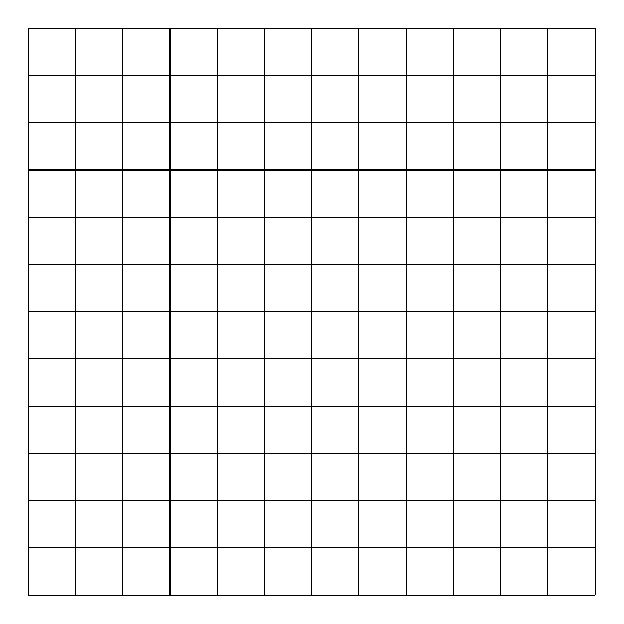
\begin{tikzpicture}[scale = 0.6]
			\draw (0,0) grid (12,12);
		\end{tikzpicture}
		\end{center}
		First, we count the horizontal blocks. There are 10 blocks per row, for a total of 120 blocks for 12 rows. Consequently, there are 120 blocks for 12 columns. There are 20 blocks for the two main diagonals. For the smaller diagonals, we have $4(1+2+3+\cdots+9)=4\times 9\times 10\div 2=180$ blocks. Therefore, there are 440 such blocks, all in all.
	\end{solution}

	\item Find the largest possible value of 
	\begin{equation}
		(\sin\theta_1)(\cos\theta_2)+(\sin\theta_2)(\cos\theta_3)+\cdots+(\sin\theta_{2013})(\cos\theta_{2014})+(\sin\theta_{2014})(\cos\theta_1).\label{eq:16}
	\end{equation}
	\begin{solution}
		The largest value of $\sin x\cos y$ is attained when $x=y=\frac{\pi}{4}$. Therefore, the largest possible value of \eqref{eq:16} is 1007.
	\end{solution}

	\item What is the remainder when $16^{15}-8^{15}-4^{15}-2^{15}-1^{15}$ is divided by 96.
	\begin{solution}
		I don't know if there are some more elegant solutions. I just performed arithmetic$\pmod{96}$ to get 31.
	\end{solution}

	\item 
	Segment $CD$ is tangent to the circle with center $O$, at $D$. Point $A$ is in the interior of the circle, and segment $AC$ intersects the circle at $B$. If $OA=2$, and $AB=4$, $BC=3$, and $CD=6$, find the length of segment $OC$.
	
	\includegraphics[width=0.25\linewidth]{PMO17_18}
	
	\begin{solution}
		Wala pa.
	\end{solution}
	
	\item Find the maximum value of 
	\begin{equation*}
		(1-x)(2-y)(3-z)\left(x+\dfrac{y}{2}+\dfrac{z}{3}\right)
	\end{equation*}
	where $x<1$, $y<2$, $z<3$, and $x+\frac{y}{2}+\frac{z}{3}>0$.
	
	\begin{solution}
		Wala pa.
	\end{solution}

	\item Trapezoid $ABCD$ has right angles at $C$ and $D$, and $AD > BC$. Let $E$ and $F$ be the points on $AD$ and $AB$, respectively, such that $\angle BED$ and $\angle DFA$ are right angles. Let $G$ be the point of intersection of segments $BE$ and $DF$. If $\angle CED = 58\degre$ and $\angle FDE = 41\degre$, what
	is $\angle GAB$?
	
	\includegraphics[width=0.4\linewidth]{PMO17_20}
	
	
	\begin{solution}
		Note that $G$ is the orthocenter. If we draw line segment $BD$, then $AI\perp BD$. 
		$\triangle ECD\simeq DBE$ so $m\angle EBD = m\angle DCE = 90-58=32$.
		
		$m\angle ABG = m\angle FGB = m\angle EGD = 90 - 49 = 41$. $m\angle FBG = 90-32=58$. $m\angle ABI=32+41=73$. $m\angle GAB = m\angle IAB = 90-73=17$.
		
		\includegraphics[width=0.6\linewidth]{PMO17_20s}
	\end{solution}
	
\end{enumerate}

\end{document}